\chapter{Implementation}

\begin{chapterabstract}
Lorem ipsum dolor sit amet...
\end{chapterabstract}

The following chapter will describe the implementation of the toolkit as envisioned in this thesis, building on the foundation created in the previous analysis and design chapters. 

Implementation focuses primarily on the requirements outlined in \autoref{requirements}, with an emphasis on those of the highest priority. The output of this chapter is the realization of a viable and usable tool.

%______________________________________________________________
\section{Structure of the toolkit}
%______________________________________________________________

The application is designed as a front-end only solution. This architecture simplifies the deployment and dependencies, making it easier to integrate into existing systems. Compared to a full stack solution, it also reduces maintenance and from a security point of view minimizes the attack surface. 

Given it's front-end nature, the configuration's administration can be done through reading from static configuration files rather than relying on data from a backend API. This way, operators of the application can easily adjust the application's behavior and offerings without the need for complex back-end processing, which is not needed in this case as the data are not sensitive or time specific and have a predefined structure. 

Consequently, the toolkit is divided into two main applications: the configurator component and the administrator component. The configurator is the user-facing part that businesses deploy or embed on their webservers, offering the ability to configure products based on the supplied configuration files. The administrator application, on the other hand, is used by the toolkit operators to generate and edit these configuration files.

It should be noted that with this architecture, deploying the administrator application is not a prerequisite for every instance of the configurator; it can be used across various configurators of the same version or even run for the necessary short while in development mode. This flexibility ensures that businesses can manage and update their configurator setups without the need to deploy an instance of the administrator application.

This architecture not only enhances the toolkit's scalability and ease of use, but also ensures that it can be easily integrated into a wide range of business environments, addressing different customization needs without the complexities and overheads associated with traditional back-end-dependent applications.

This structure is also implemented in such a way that if the need for a back-end develops one day, it will be very easy to modify the application for that change.

% - - - - - - - - - - - - - - - - - - - - - - - - - - - - - - -
\subsection{Project directory tree}
% - - - - - - - - - - - - - - - - - - - - - - - - - - - - - - -

\dirtree{%
.1 /.
    .2 apps/.
        .3 admin/.
            .4 src/.
            .4 index.html.
            .4 vite.config.ts.
            .4 package.json.
        .3 main/.
            .4 src/.
            .4 index.html.
            .4 vite.config.ts.
            .4 package.json.
    .2 packages/.
        .3 shared/.
            .4 src/.
            .4 package.json.
    .2 package.json.
}
\vspace{16pt}

Given the separation of the toolkit into the configurator and administrator components, the project is split into two subprojects in the \texttt{apps} directory. The configurator application is located in the main directory, while the admin directory contains the source files for the administrator application. Consequently, each of the subprojects has its own Vite configuration, among their \texttt{index.html} files, \texttt{src} directories for code and \texttt{package.json} for managing the subproject-specific dependencies. 

To minimize code duplication, the \texttt{shared} library is located in the \texttt{packages} directory. This shared library contains common elements imported by both applications, such as data schemes, generic React components, custom React hooks, types and interfaces, CSS styles, or other utility functions. Using this shared package in the configurator and administrator applications ensures consistency and reduces redundancy across the toolkit.

Most dependencies are managed centrally in the root \texttt{package.json} file, with dependencies specific to the subprojects being handled in their corresponding package files. This approach optimizes dependency management across the entire project.

It is important to note that the presented directory tree focuses on illustrating the separation of the project into subprojects: configurator and administrator applications, and the shared library. It is not exhaustive, as the actual project contains various other config and dot files.

The following is a brief overview of the \texttt{src} directories, which organize the source code into logical sections. The directories have the same layout across all subprojects.

\vspace{12pt}
\dirtree{%
.1 src/.
    .2 components/\DTcomment{UI elements, React components}.
    .2 configurations/\DTcomment{configuration of the application}.
    .2 hooks/\DTcomment{custom React hooks}.
    .2 interfaces/\DTcomment{object interfaces}.
    .2 schemas/\DTcomment{data schemas}.
    .2 stores/\DTcomment{data stores and actions}.
    .2 styles/\DTcomment{CSS styles}.
    .2 toasts/\DTcomment{presets for toasts (notifications on top of screen)}.
    .2 utilities/\DTcomment{helper functions and classes}.
}
\vspace{16pt}

\todo{Unimplement baseSpec in code, reference productspecification in usercreation, change size in MaterialSpecification in UML, change color of materials and mounted in UML, rename catalogue to catalog everywhere, add optional attributes in uml, id an product schema}

%______________________________________________________________
\section{Data schemas}
%______________________________________________________________

The data schemas are derived from the domain model discussed in \autoref{section:domain-model}. These schemas define the shape of the objects that are used to transfer and store information within the tool. 

To visualize these schemas, a UML diagram is provided in \autoref{fig:data-schema}. The diagram provides a general overview of utilized the structures and associations, but the implementation requires slight adjustments.

Data schemas are stored in the shared library discussed in the previous section. This ensures consistency, as they are used in both the main and admin applications. 

The schemas are organized into three separate parts: Catalog, product specification, and user creation. Each of these parts corresponds to a separate file in the shared library, in addition to their different roles within the application. The parts are discussed in the following sections, and the UML diagram in \autoref{fig:data-schema} provides color coding to differentiate them.

As discussed in \autoref{section:zod}, the implementation of data schemas utilizes the Zod validation library, which allows straightforward validation of the shape of the data during parsing. TypeScript types are then easily created from these Zod schemas, which is illustrated in \autoref{listing:zod}. \cite{Wycliffe2023} 

\begin{landscape}
\begin{figure}[h]
\centering
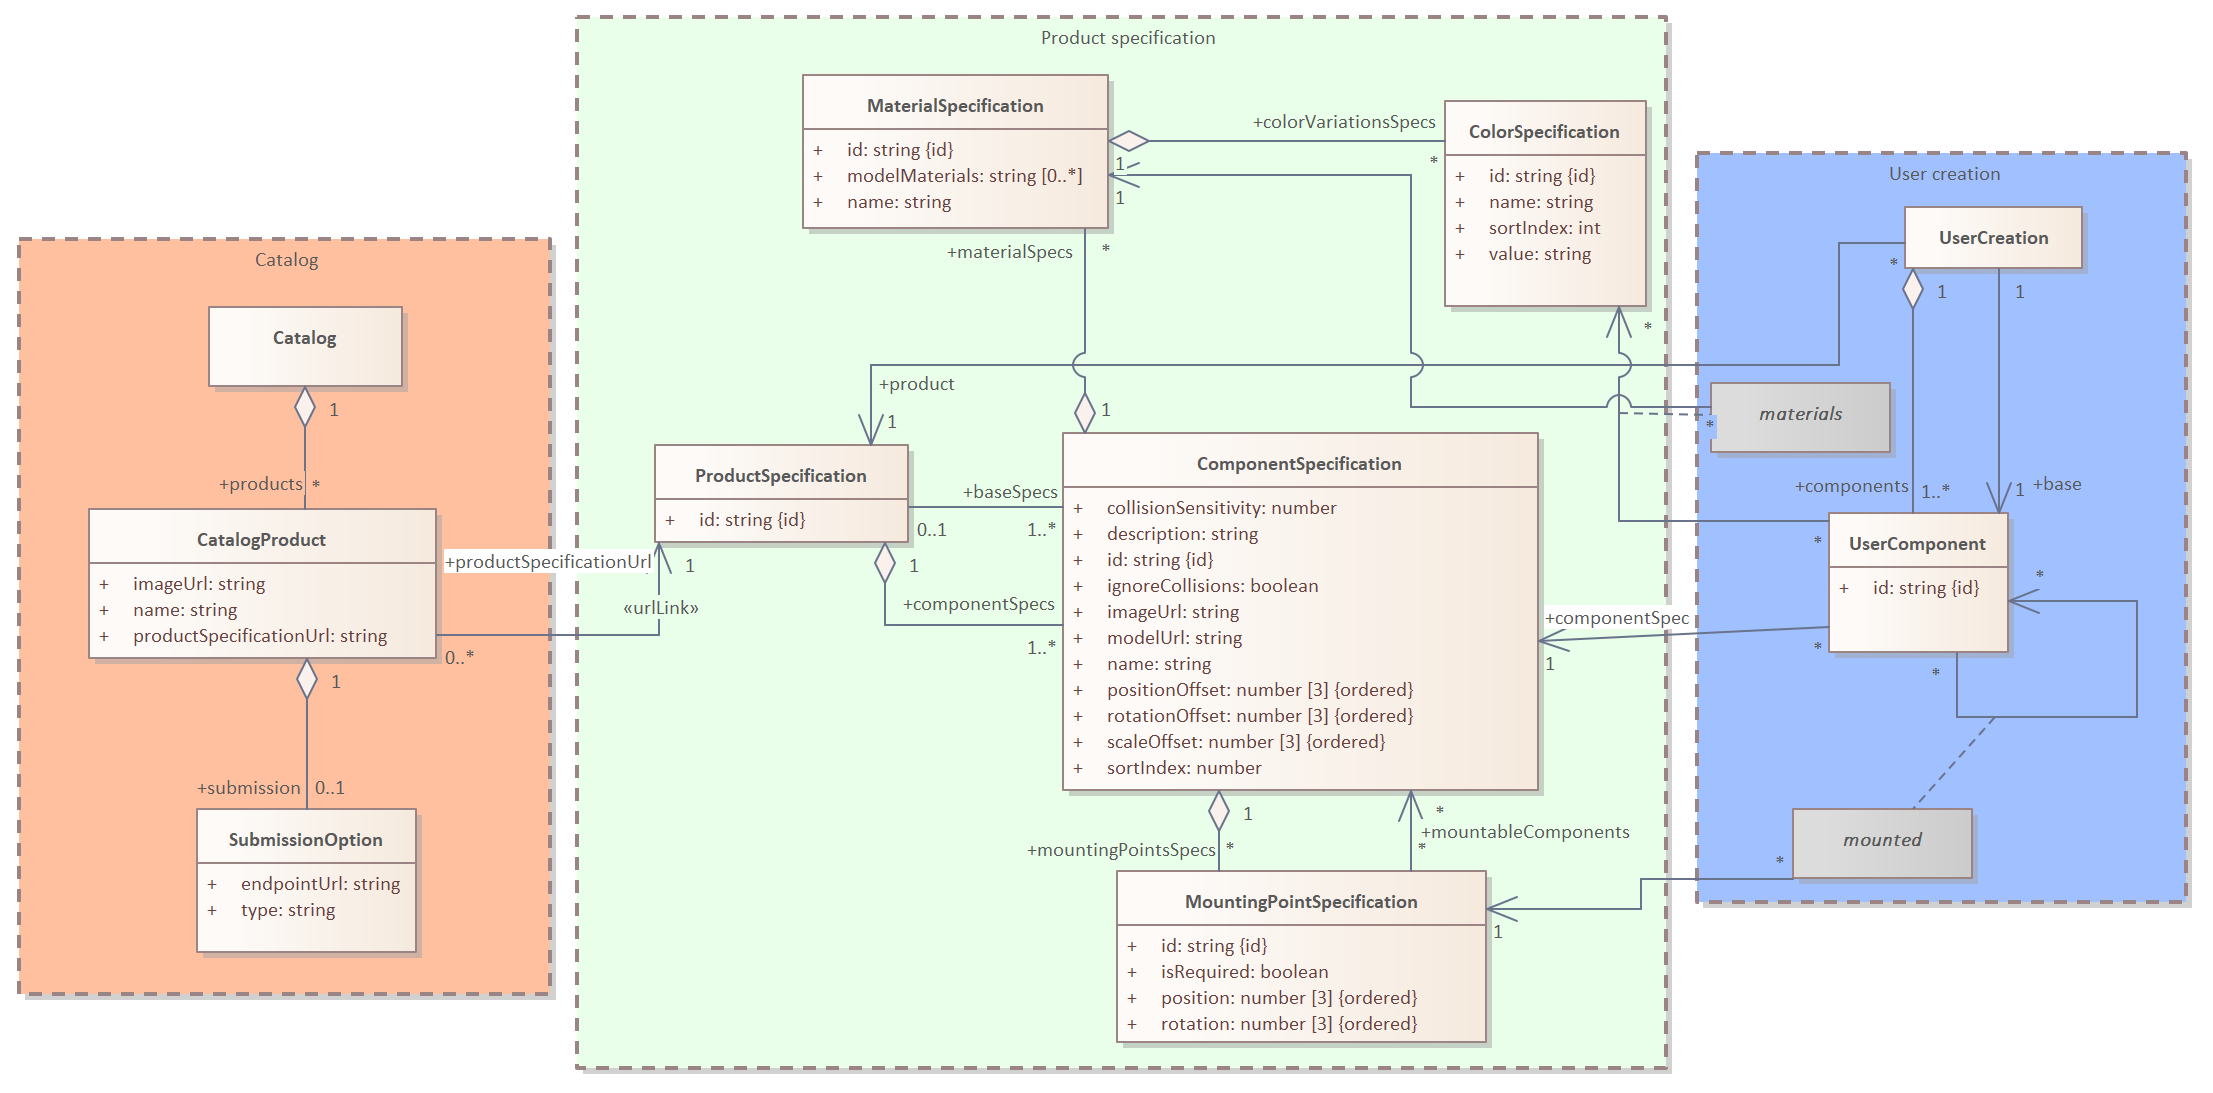
\includegraphics[width=\linewidth]{images/uml_dataschema.png}
\caption{Data schemas as a UML diagram}
\label{fig:data-schema}
\end{figure}
\end{landscape}

% - - - - - - - - - - - - - - - - - - - - - - - - - - - - - - -
\subsection{Catalog}
% - - - - - - - - - - - - - - - - - - - - - - - - - - - - - - -

The catalog data schema, visualized with an orange tint in the UML diagram, is essential for the initial user interaction with the application.

\begin{listing}[h]
\begin{minted}{text}
export const SubmissionOptionSchema = z.object({
  type: SubmissionTypeSchema,
  endpointUrl: z.string().url(),
});

export const CatalogueProductSchema = z.object({
  name: z.string().max(100),
  productSpecificationUrl: z.string(),
  imageUrl: z.string(),
  submission: SubmissionOptionSchema.optional(),
});

export const CatalogueSchema = z.object({
  products: z.record(CatalogueProductSchema),
});
\end{minted}
\caption{Data schema of catalogue}
\label{lisiting:schema-catalogue}
\end{listing}

Building upon the domain model, the catalog is created by the operator of the tool and covers all product specifications. However, compared to the domain model, there is an additional level of abstraction in the form of \texttt{CatalogueProduct}, which contains the most important information about the product specification, such as the name and the preview image. The catalog is separated from the product specifications, which are stored elsewhere. One reason for this is that the catalog will first be fetched when the configuration application is launched, and this information must be presented to the user as soon as possible. The specification of the product, which contains the information needed for the configuration process, can then be fetched from an URL stored inside this object after the user decides which product to configure, which is represented by the stereotype \texttt{urlLink} in the UML diagram.

In addition, each product stores information about the confirmation action in the form of a \texttt{SubmissionOption}, which specifies the type of action and the endpoint to which the application potentially sends the confirmed configuration.

The TypeScript implementation can be seen in \autoref{lisiting:schema-catalogue}. In the catalogue, each product is stored using a record structure, with ID of the product as a key. The names have been arbitrarily limited to 100 characters to ensure that they can fit within the correct user interface position. URLs, except for the endpoint, are not validated to accommodate local addresses.


% - - - - - - - - - - - - - - - - - - - - - - - - - - - - - - -
\subsection{Product specification}
% - - - - - - - - - - - - - - - - - - - - - - - - - - - - - - -

The advantage of the structure where the catalog is separate from the specifications, which are fetched only when needed, is that each specification can be sourced from a different location. The specifications can also be updated independently on the rest of the catalog.

The product specification part is visualized by a green tint in the UML diagram.  

\begin{listing}[h]
\begin{minted}{typescript}
export const ComponentSpecificationSchema = z.object({
  name: z.string().max(100),
  description: z.string(),
  imageUrl: z.string(),
  modelUrl: z.string(),
  materialSpecs: z.record(
    MaterialSpecificationSchema
  ),
  mountingPointsSpecs: z.record(
    MountingPointSpecificationSchema
  ),
  positionOffset: z.tuple(
    [z.number(), z.number(), z.number()]).optional(),
  rotationOffset: z.tuple(
    [z.number(), z.number(), z.number()]).optional(),
  scaleOffset: z.tuple(
    [z.number(), z.number(), z.number()]).optional(),
  ignoreCollisions: z.boolean().optional(),
});

export const BaseSpecificationSchema = z.object({
  component: z.string(),
});

export const ProductSpecificationSchema = z.object({
  baseSpecs: z.record(BaseSpecificationSchema),
  componentSpecs: z.record(ComponentSpecificationSchema),
});
\end{minted}
\caption{Data schema of product and component specifications}
\label{lisiting:schema-componentspecification}
\end{listing}

This part of the data is created by the tool's operator and provides information about the available options for user configuration of a chosen product.

The schemas are also derived from the domain model, although with some modifications such as changes in attributes and some objects being merged.

Most of the concepts in this part are identical to the domain model; however, the new concept of \texttt{base} component is introduced here. Due to the modularity principle, each component is in some way mounted on another component. Base components are such components that can initiate the configuration as they are not mounted to other components. They represent the potentially first component of a configuration. These base components are defined in the product specification.

In the data schema, the model is directly included in the component specification, with the \texttt{modelUrl} attribute pointing to a location with the 3D model file. To compensate for this coupling, attributes that modify the position, rotation, and scale of the model are added to the component specification. Further attributes are also present, such as a description or the option to ignore collisions for this component. The material specification includes the names of the model's meshes in the attribute \texttt{modelMaterials}, and the color specification features the \texttt{sortIndex} attribute, which determines the presentation order to the user.

In TypeScript, the aggregations depicted in the UML diagram are implemented as records, with the IDs serving as keys and the objects as values. Other associations are implemented using solely IDs. Color values are represented using hex code. The implementation of the product and component specifications can be viewed in \autoref{lisiting:schema-componentspecification}. Other entities in this section are implemented similarly and therefore do not require detailed previews within the text of the thesis.


% - - - - - - - - - - - - - - - - - - - - - - - - - - - - - - -
\subsection{User creation}
% - - - - - - - - - - - - - - - - - - - - - - - - - - - - - - -

\begin{listing}[h]
\begin{minted}{typescript}
export const UserComponentSchema = z.object({
  componentSpec: z.string(),
  materials: z.record(z.string()),
  mounted: z.record(z.string()),
});

export const UserCreationSchema = z.object({
  base: z.string(),
  components: z.record(UserComponentSchema),
});
\end{minted}
\caption{Data schema of user creation}
\label{lisiting:schema-usercreation}
\end{listing}

User creation corresponds to the configuration entity of domain model, but has been renamed in implementation, as \texttt{configuraiton} is an ambiguous term that can mean several things in application development, for example configuration of the application itself. This makes it clearer what this data schema is representing.

User creation is tinted blue in the UML diagram.

User creation stores the configured components, as well as the selected base component, which is the first component of the configuration. All other components are mounted on this component or other components.

In contrast to the domain model, the configured component is represented by \texttt{UserComponent}. This configured component links to a component specification that serves as a template. It also stores information about the mounted components, including the specific mounting points where each component is attached, as well as the selected colors of the materials that have been customized.

In the TypeScript implementation, which can be viewed in the \autoref{lisiting:schema-usercreation}, the user components are stored in a record with their unique ID as the key. The component specification for each user component is linked by its ID. Information about mounted components are stored in records, with the mounting point specification ID as the key to identify the position and the ID of the user component as the value. Similarly, materials are organized with the material specification ID as the key and the ID of the selected color specification for that material as the value.


%______________________________________________________________
\section{Challenges and solutions}
%______________________________________________________________

During the implementation phase of the project, various challenges emerged. This section touches on these challenges, detailing both the issues encountered and the innovative solutions used to overcome them. The majority of these challenges were related to the implementation of the defined requirements. Examining these obstacles offers valuable insight into the software engineering involved in the development of product configurators.


\subsection{Component visualization}

The implementation of component visualization primarily stems from requirement \hyperref[itm:F1]{F1}, which mandates a 3D visualization of the configured product while employing realistic models. The solution is shaped by the chosen 3D technology (see \autoref{section:3Dvistech}), primarily R3F library supported by Three.js, and the created data scheme described in the previous section.

\begin{listing}[h!]
\begin{minted}{typescript}
export const Component = ({ componentId }) => {
  const { 
    component, componentSpec
  } = useComponent(componentId);

  return (
    <group name={componentId
    }>
      <ComponentModel componentId={componentId} />

      {Object.entries(componentSpec.mountingPointsSpecs).map(
        ([mountingPointSpecId, mountingPoint]) => {
          const mountedComponentId = component
            .mounted[mountingPointSpecId];

          return (
            <group
              key={mountingPointSpecId}
              position={mountingPoint.position}
              rotation={mountingPoint.rotation}
            >
              {mountedComponentId ? (
                <Component componentId={mountedComponentId} />
              ) : (
                <MountingPointButton
                  componentId={componentId}
                  mountingPointSpecId={mountingPointSpecId}
                />
              )}
            </group>
          );
        }
      )}
    </group>
  );
};
\end{minted}
\caption{Implementation of component visualization}
\label{lisiting:impl-visulaization1}
\end{listing}

A simplified version of the implementation is illustrated in \autoref{lisiting:schema-componentspecification}. The group feature of R3F library is utilized for effective position and rotation composition. The component is primarily made up of this group, which integrates the model and the mounting points of the component.

Inside \texttt{ComponentModel}, the 3D model is loaded from a GLTF file, a format which can fully represent 3D objects widely used in web applications and greatly supported in the Three.js library. The position, rotation and scale of the model is adjusted by the values stored in the component specification, using a nested R3F group, which can be previewed in \autoref{lisiting:impl-modelcomposition}.

Considering that configured components (other than the base) are mounted on top of each other, a recursive approach is employed to manage this hierarchical structure and mapping between the data schema and the visualization. Therefore, for each mounting point defined in the component specification, a nested group is utilized to adjust the position and rotation according to the mounting point specification. If a component is attached to this mounting point, it is recursively inserted into the group; otherwise, a spatial button is displayed at this place to facilitate the addition of the component. 

This recursive nesting ensures that each mounted component's position and rotation are automatically adjusted through the group composition, eliminating the need for direct calculation of these values. The simplification this offers significantly outweighs the minor performance impact introduced by recursion.

Properties are managed through Valtio proxies using custom hook \texttt{useComponent}, therefore whenever the underlying state changes, the interface including the 3D elements immediately redraws.
All components are placed within an R3F \texttt{canvas} element. The orbital camera controls needed by the requirement \hyperref[itm:F2]{F2} are done using \texttt{OrbitControls} Three.js element integrated using Drei library, which is placed within the canvas and offers standard orbital camera controls.

\subsubsection{Component interactivity}

To meet the requirement \hyperref[itm:F4]{F4}, which enables users to select components directly within the visualization, an \texttt{onClick} event is utilized on the group containing the model. Upon clicking a component, a side panel is presented that displays detailed information about the selected component. To visually highlight the selected component in the visualization, an outline of the model is created using the \texttt{Edges} element from the Drei library, which is included within the same group as the model. The color of the outline can be configured by the application administrator. Additionally, an \texttt{ onPointerMissed} event employed on the canvas allows to deselect the component by clicking on the background.

\subsection{Model material change}

To fulfill the requirement \hyperref[itm:F8]{F8}, which allows users to modify the appearance of materials in a component, there must be a mechanism that allows the colors of parts of the model to be changed within the preview. Each GLTF file with model contains meshes and default materials. When the user changes the color of a material, the model needs to be decomposed into its atomic parts. This allows for each part's material to be found and adjusted. 

In the implementation, which is in a simplified form presented in \autoref{lisiting:impl-modelcomposition}, it is iterated through all meshes and materials of the model, replacing the default materials for the customized ones whenever needed. As a result of this approach, the model is not inserted into the scene at once, but instead every mesh is included separately along with the corresponding material. This is achieved using the group where all the meshes of the model reside, which as mentioned in the previous section also changes the position, rotation, and scale of the model.

Changing the colors of the materials is facilitated through the side panel. The new color value is stored in a Valtio proxy, from which it is read when composing the 3D model, ensuring dynamic updates of the visual preview whenever the user makes changes.

\begin{listing}[h!]
\begin{minted}{typescript}
<group
  onClick={onSelect}
  position={componentSpec.positionOffset}
  rotation={componentSpec.rotationOffset}
  scale={componentSpec.scaleOffset}
>
  {Object.entries(model).map(([name, node]) => {
    if (node.type === "Mesh") {
      const mesh = node as Mesh;
      const material =
        customMaterials[mesh.material.name] 
        || materials[mesh.material.name];

      return (
        <mesh
          key={name}
          geometry={mesh.geometry}
          material={material}
        />
      );
    }
  })}
</group>
\end{minted}
\caption{Implementation of model composition}
\label{lisiting:impl-modelcomposition}
\end{listing}

\subsection{Undo and redo actions}

Undo and redo actions enable users to revert the changes made during the configuration process, fulfilling the requirement \hyperref[itm:F13]{F13}. Buttons for these actions are intuitively designed as forward and backward arrows and are placed around the preview view.

Since the user's creation is stored in a Valtio proxy during the configuration process, the implementation of this feature is straightforward. Valtio provides an enhanced version of the proxy that maintains a history in the form of snapshots and includes callable undo and redo functions. The management of snapshots is smart, as multiple actions performed immediately after each other are considered to be aggregated within one snapshot. This is particularly useful for this application, since, for example, the addition of a new component consists of two operations: the creation of a new component in the store and then mounting it on a point on another component, which is correctly considered as only one snapshot. Therefore, except for the setup of the initial snapshot, this implementation approach did not need any additional adjustments.

\subsection{Collision detection}

Collision detection is necessary for preventing impossible configurations by disallowing physically overlaping components. This feature directly addresses the requirement \hyperref[itm:F7]{F7}. As the shapes of the components can be highly complicated, the method for detecting collisions needs to be based on the 3D preview working directly with the component models.

Three.js provides a bounding-box method (where each model is considered to be cube shaped, and overlaps are determined based on these primitive shapes), which is far too simple for complex shapes and large amounts of models; therefore, a more sophisticated approach was needed. 

The three-mesh-bvh package extends the Three.js library by providing an implementation of a bounding volume hierarchy (BVH) tree, which enables efficient shape intersection queries for high-definition meshes. \cite{Johnson2023}

To compute the bounds tree, the entire scene is wrapped in a \texttt{bvh} element from the Drei library, which performs this computation on each mesh. Collision detection is performed for all mountable components at every unoccupied mounting point whenever there are additions or removals of user-created components or when attempting to swap the configured component. To do so, the model of the component is loaded, adjusted by values in component specification, and its position is set to the potential mounting location in the scene. This is not visible in the preview to the user and is performed using standard Three.js code. 

Then, each mesh of the model is queried on geometry collision against the meshes of existing components in the preview, excluding the component containing the mounting point. This exclusion happens because, when a mounting point exists, even if there is a collision with the owning component, all defined mountable components should be allowed to be mounted. In addition, the administrator of the tool can exclude certain type of components from all collision calculations by specifying this in the component specification. Collision sensitivity can also be adjusted for each component specification. Setting this option to low sensitivity causes the loaded model that is checked for collisions with the scene to be slightly reduced in size, meaning close fits are more likely to pass.

In case the model collides with existing components in the scene, the option to add the component to the configuration is not presented to the user.

A highly simplified implementation that illustrates this principle can be seen in \autoref{lisiting:impl-collisiondetection}. Although the collision detection is highly computationally intensive, it is performed only after specific user actions, which are not supposed to be very frequent; therefore, the possible performance hit is deemed acceptable given its benefits.

\begin{listing}[h!]
\begin{minted}{typescript}
export function collisionDetection(
  model: THREE.Group,
  scene: THREE.Scene
): boolean {
  const collisionDetected = false;

  traverseMeshes(model, (modelMesh) => {
    traverseMeshes(scene, (sceneMesh) => {
      const transformMatrix = new THREE.Matrix4()
        .copy(sceneMesh.matrixWorld)
        .invert()
        .multiply(modelMesh.matrixWorld);

      if (
        (sceneMesh.geometry as BVHBufferGeometry)
          .boundsTree.intersectsGeometry(
            modelMesh.geometry,
            transformMatrix
          )
      ) {
        collisionDetected = true;
      }
    });
  });

  return collisionDetected;
}
\end{minted}
\caption{Implementation of collision detection}
\label{lisiting:impl-collisiondetection}
\end{listing}

\subsection{Configuration confirmation}

For the implemented tool to be useful, there needs to be a mechanism that will facilitate performing further actions with the user's configuration when the configuration process finishes. This is in accordance with the requirement \hyperref[itm:F10]{F10}.

As needed by requirement \hyperref[itm:F9]{F9} and discussed previously, after completion of the product configuration, users are presented with a summary screen that details the selected options. To save the configuration for future reference in a readable way, a button has been introduced that enables saving this summary to PDF. Implementation of this button action needed to be done on the front-end and utilizes the HTML print API.

\begin{listing}[h!]
\begin{minted}{typescript}
export const ContactInfoSchema = z.object({
  name: z.string(),
  email: z.string().email(),
  phone: z.string().max(20).optional(),
  note: z.string().max(10000).optional(),
});
\end{minted}
\caption{Data schema of contact information}
\label{listing:schema-contactinformation}
\end{listing}

The administrator of the tool can define the confirmation action in the catalog. If such an action is defined, it must include an endpoint URL to ensure that these actions can be executed. The supported confirmation actions are as follows:

\begin{enumerate}
    \item \textbf{Preview}: This is the default behavior if no confirmation action is defined. In this case, the confirmation button is not presented to the user at all, and the configurator serves only as a preview tool. The URL of the endpoint is also not defined.
    \item \textbf{Redirect}: This action allows for a simple flow where clicking the confirmation button redirects the user to the chosen URL.
    \item \textbf{POST request}: Upon clicking the confirmation button, the user configuration, in the form of the user creation data schema presented in the previous sections, is sent using a POST request to the defined endpoint URL. The user creation is sent as a JSON in the body of the request. In order to present the result of this action as a success to the user, the response must return OK. Optionally, the response can contain a JSON body with valid URL as the \texttt{redirectUrl} field. If this is the case, and the request has been successful, users will be redirected to this returned URL, otherwise, the tool returns to the initial view. This mechanic facilitates possible integration with back-end systems or serverless functions for further processing.
    \item \textbf{Inquiry form}: This action presents the user with an inquiry form asking for their contact information, such as name, email, phone number, and additional notes. This fulfills the requirement \hyperref[itm:F11]{F11}. When the form is sent, the process is identical to the POST request case, with the difference that the request contains the user contact details in the JSON payload under the field \texttt{contact}. This allows for direct creation of inquiries without the need for users to navigate away from the application. The structure of the contact data schema is detailed in \autoref{listing:schema-contactinformation}.
\end{enumerate}


\subsection{Application configuration}

Application configuration is central for setting the behavior and appearance of the tool so that the individual preferences of the operator are met. Given that the solution is designed for adaptability, it is essential to provide extensive setup options. These settings are managed by the administrator of the application, allowing them to tailor the application without the need to change the code directly. This also helps to fulfill the interface customization requirement \hyperref[itm:F14]{F14}.

\begin{listing}[h!]
\begin{minted}{typescript}
fetch(globalConfigUrl)
  .then((response) => {
    return response.json();
  })
  .then((data) => {
    globalConfig.config = AppConfigSchema.parse(data);
  })
  .then(() => {
    ReactDOM.createRoot(document.getElementById("root")!)
        .render(<App />);
  })
  .catch((error) => {
    console.error(error);
    ReactDOM.createRoot(document.getElementById("root")!)
        .render(
            <p className="text-red-600">
              Fatal error: couldn&apos;t initialize appconfig.
            </p>
        );
  });
\end{minted}
\caption{Implementation of application initialization and config loading}
\label{listing:impl-applicationconfig}
\end{listing}

As the tool is front-end-based, its configuration is handled using a JSON file. The file is fetched at the start of the application, before React is even initialized, from location \texttt{/appconfig.json}. This ensures that the configuration is not baked in the application, rather it is refreshed each time the application is accessed, meaning that the administrator can update the settings without the need to redeploy the entire application, which supports the maintainability requirement (\hyperref[itm:NF5]{NF5}). The implementation of the application initialization with the fetch of the config can be seen in \autoref{listing:impl-applicationconfig}.

The config file includes the URL with the location of catalog (which is therefore also fetched at runtime, allowing for live updates), toggles for features, settings of the 3D preview, and color settings for the tint of the interface, meaning unless larger customization is required, there is no need for CSS modifications. It also includes locations of images such as logos or favicons, as well as the title of the website.

\subsubsection{Interface texts}

As described in \autoref{section:i18n}, the i18next library was chosen for localization. This addresses the multilingual support requirement (\hyperref[itm:NF8]{NF8}), as well as simplifies the interface text customization requirement (\hyperref[itm:F15]{F15}).

The library is setup in such a way that it expects for all localization files to be located in \texttt{/locales/\{language\}/translation.json}, where \texttt{\{language\}} is a two-letter language code. This structure allows simple addition of further languages without impact in rest of the tool functionality, as the applicaiton performs automatic lookup for these translation files. One language needs to be designated as the default localization in the general config file, which serves as the fallback.

Like the the general config file, the translation files are loaded at runtime, therefore changes to the interface texts or additions of new localizations can be performed without redeploying of the application.

The application attempts to automatically choose the correct language based on the detected browser settings, but also allows users to override this selection via a two-letter parameter in the \texttt{?lng=} query of any URL in the application.  

As part of the implementation, a default template localization in English is provided, providing a baseline.

\subsection{Routing}

Routing within the application is performed using the React Router library, based on a choice discussed in \autoref{section:react-router}.

Routes are split based on the three main screens designed using wireframes in \autoref{section:wireframes}. The routing pattern is implemented as follows:

\begin{itemize}[label=\rectanglebullet]
    \item Route \texttt{/} navigates to the introductory screen
    \item Route \texttt{/editor/:productId} navigates to the screen with the configuration process itself. The parameter of product ID denotes the product int the catalog.
    \item Route \texttt{/confirm/:productId} navigates to the confirmation screen using the same product ID as in the configuration process.
\end{itemize}

Routing helps the user navigate the application better, as forward and backward browser actions are possible, meaning that users can return from the confirmation screen to the configuration screen by clicking back; this means that the browsing history is preserved. Navigation between screens occurs without page refreshes, maintaining a seamless user experience.

From an implementation standpoint, the utilization of different screens is also simplified, as they are managed centrally by the router, and are defined declaratively. 

Errors are handled by the router as well, as if there is any issue that throws an unrecoverable error during the runtime of the application, it is intercepted by the router and an error screen is displayed.

\subsubsection{Data flow}

As the application follows a specific flow between the three routes during usage, there is also some data manipulation closely tied to this. Data flow is managed by the loader functions that are executed when accessing each route. This is necessary to ensure that the application handles transitions smoothly and maintains data integrity throughout the user's session.

In the introductory screen route, the catalog is fetched into the memory to allow users to choose which product to configure.

The configuration screen route fetches the product specification based on the ID specified within the route and prepares the user creation. In case the introductory screen is not opened and users navigate directly to this route, the catalog is fetched beforehand, as well to ensure that all necessary data is available.

Furthermore, in the confirmation screen route, it is verified that some user configuration with this product ID was created. If not, the user is redirected to the configuration screen. 

The error screen is displayed if there are any discrepancies during the routing process, such as if the route requests a product that does not exist in the catalog.

\subsection{Catalog management} \label{section:catalog-management}

As outlined in the previous sections, the toolkit is structured into two separate applications: the user-facing configuration and the administrator application. This approach aligns with requirement \hyperref[itm:F16]{F16}, which demands that catalog management should be visual rather than relying on direct file editing, and should mirror the preview visible during the configuration process. Furthemore, this also addresses the requirement \hyperref[itm:F17]{F17}, so that the properties of the products within the catalog are easily manageable.

The administrator application is organized into two screens, each tailored for specific management tasks, which is reflected in its routing patterns, which are as follows:
\begin{itemize}[label=\rectanglebullet]
    \item Route \texttt{/catalogcomposer} and \texttt{/} navigates to a catalog composer screen, which provides a interface for editing the catalog data schema. In essence, it serves to modify the JSON file that contains the catalog using a visually appealing and user-friendly approach. The interface is based on structured forms that, compared to composing the file manually, enhance the efficiency and prevent errors. 
    
    \item Route \texttt{/productcomposer} navigates to a product composer screen that serves to set up component specifications and their properties. The interface of product composer aims to mirror the interface of the main application during the configuration process, but has an additional side panel on the left, which is utilized to add and remove component specifications. Selecting a component specification displays its model in the 3D preview area, while the side panel, which is used during the configuration process to present detailed information, offers settings for all attributes of the component specification, such as position, rotation, scale, mounting points, and materials.
\end{itemize} 
    
For visual editing of positioning within the product composer's 3D preview, Drei's \texttt{PivotControl} is used, which displays interactive three-axis arrows for adjusting position and rotation of the component specifications. Interacting with this control immediately stores the new values in the underlying Valtio proxy, meaning the changes are immediately reflected in both the 3D preview and the side panel, where the corresponding values are displayed in input fields. 

Given that no back-end has been implemented, the administrator application does not feature a save button. Instead, the capability to export the relevant JSON files containing the specified data schemas is provided. In addition, import of these already existing files is also possible, which provides flexibility and eases modifications.

The admin application is used when administrators need to update configuration specifications or manage catalog settings. The implementation is done in such a way that future back-end integration tying the main and administrator applications should be possible if the need and opportunity arise.


%______________________________________________________________
\section{Views}
%______________________________________________________________

This section presents the visual aspect of the implemented views and screens, which are based on the wireframes described in \autoref{section:wireframes}. The implemented interfaces are shown using screenshots, providing a visual confirmation of the design's adherence to the designed wireframes and demonstrating the application of the design concepts discussed earlier.

The choice of technologies (such as TailwindCSS) was paramount to this task, as it greatly facilitated the straightforward implementation of responsive design, making sure that the application performs well across a variety of device sizes and resolutions, as well as the accessibility features, such as automatic support for dark mode.

\subsection{Configurator application}

In the following section, screenshots of the three screens that were described using the wireframes are displayed. The interface is shown only in its light-mode version, given that the dark mode is identical, only with an inverted color scheme.

\subsubsection{Introductory screen}

\begin{figure}[h]
\centering
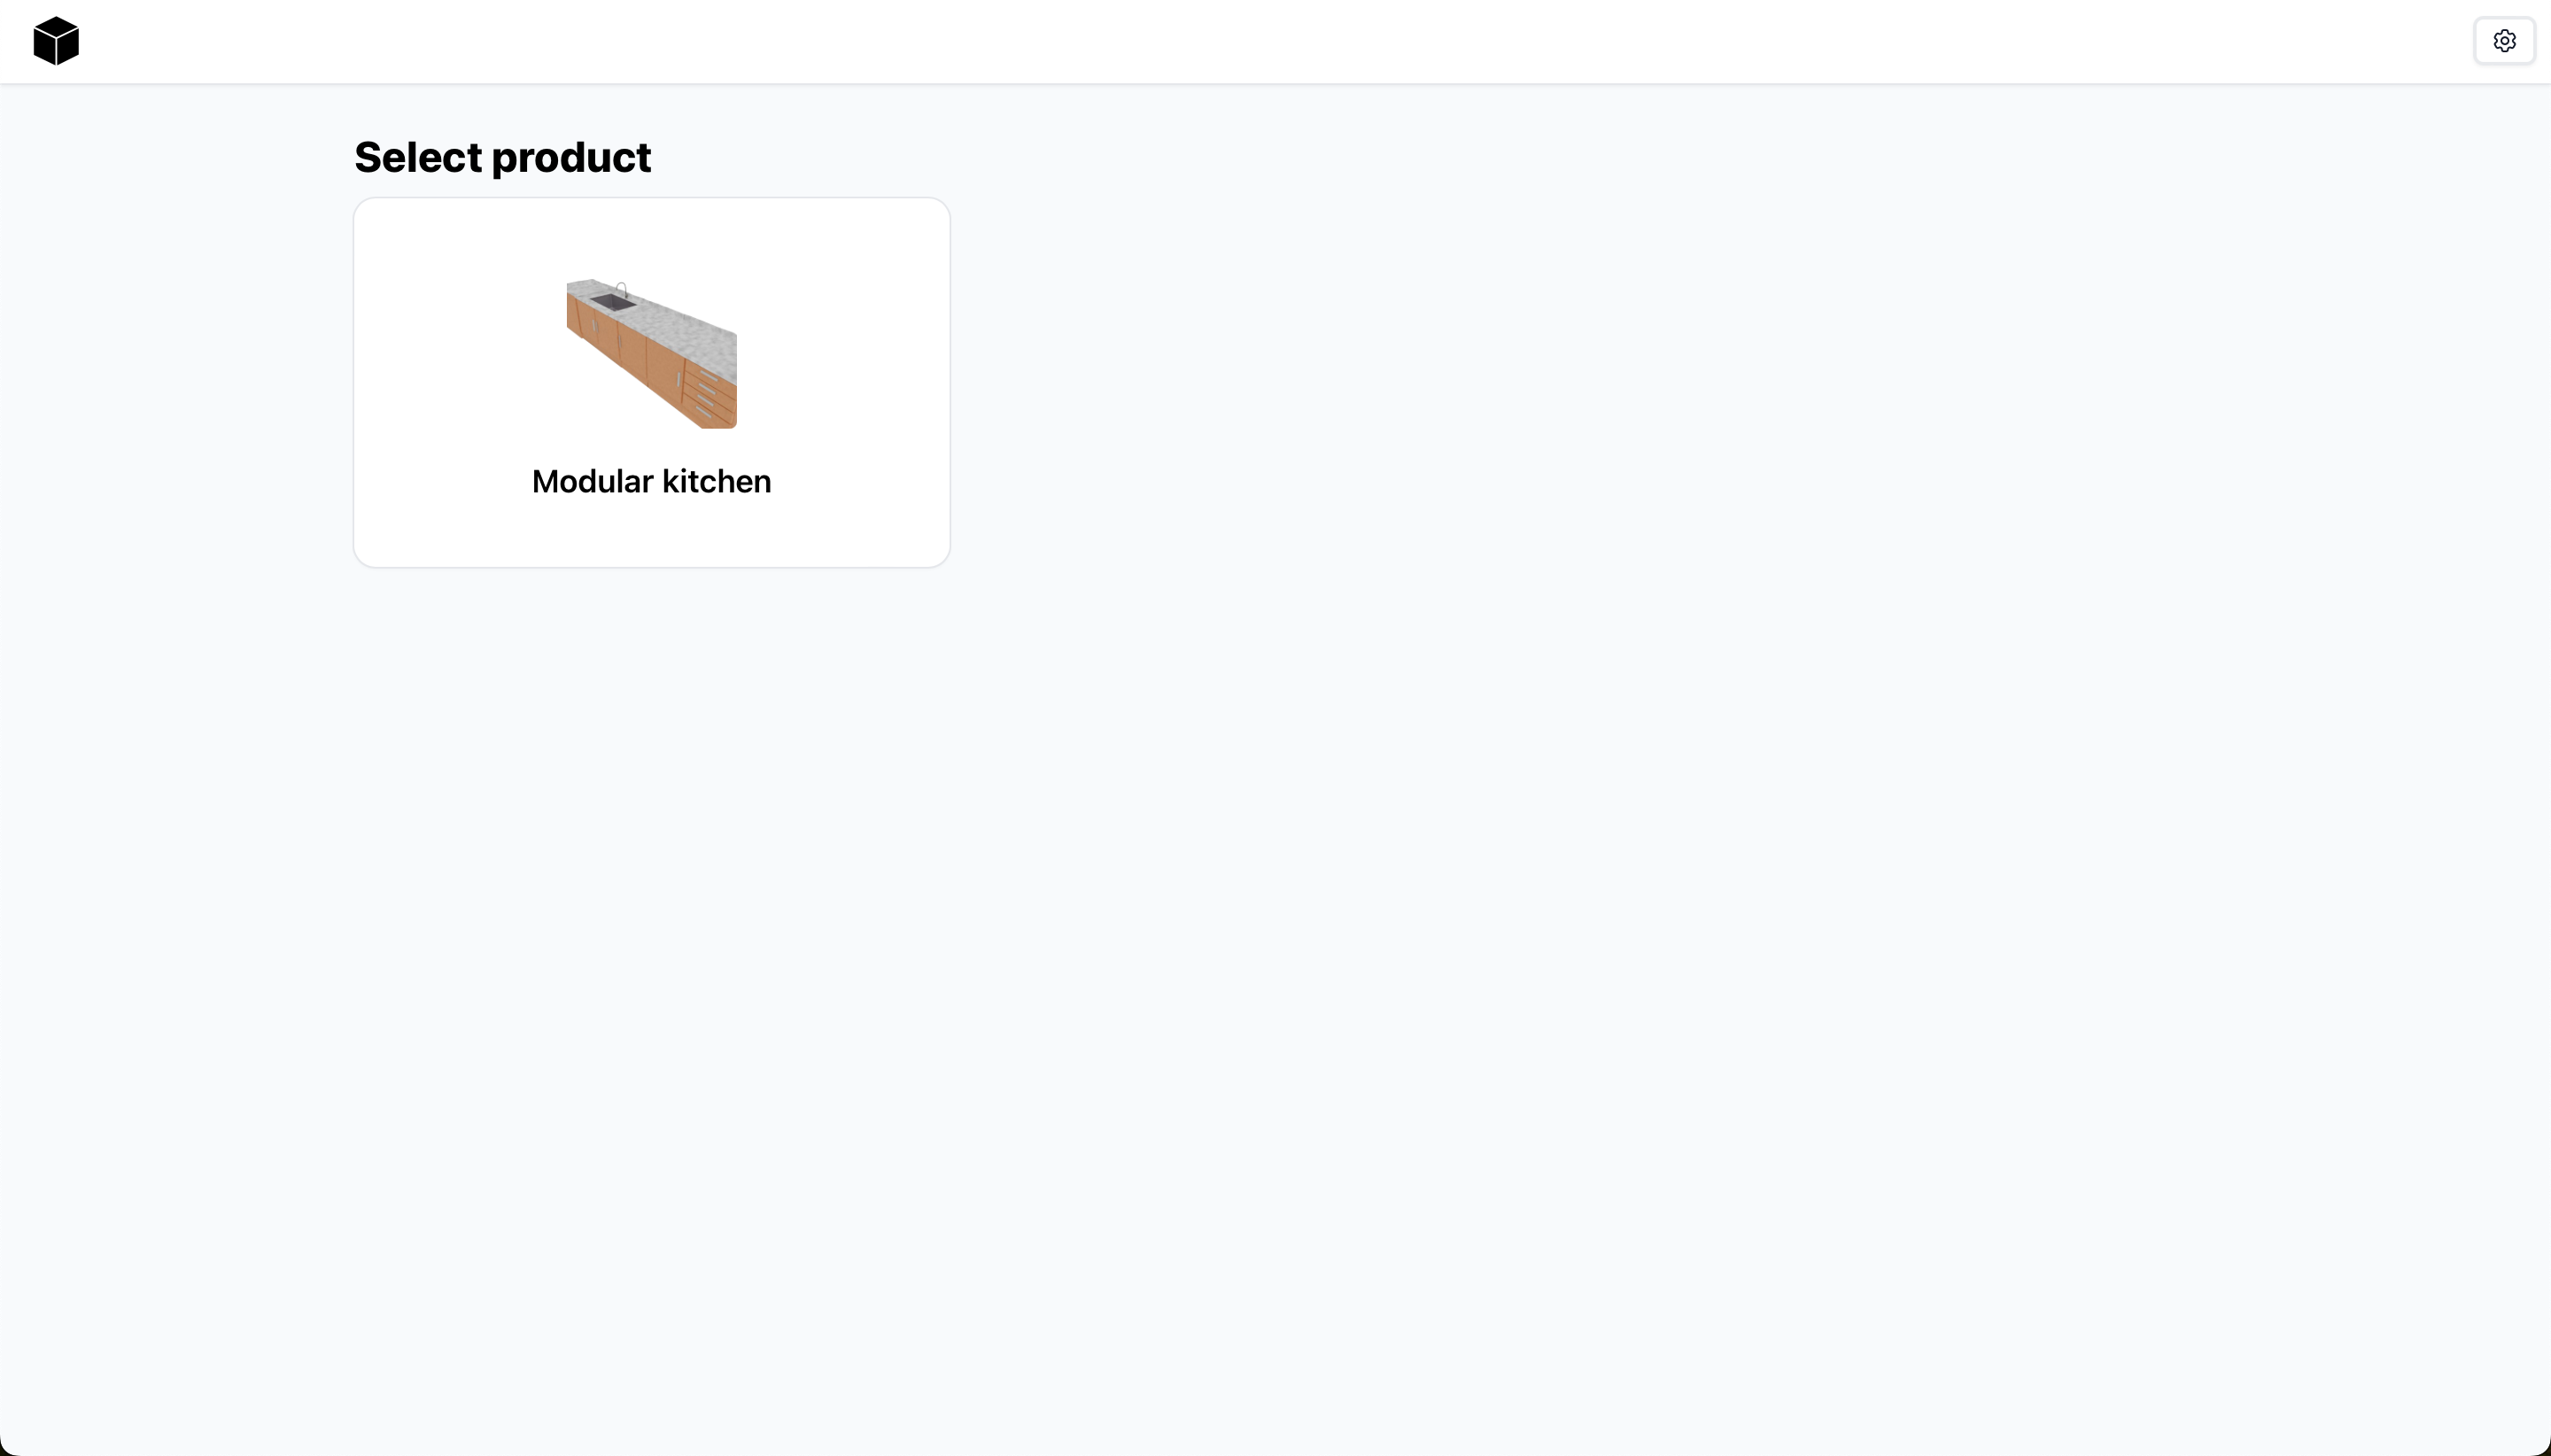
\includegraphics[width=\textwidth]{images/screenshot_introduction.png}
\caption{Screenshot of introduction screen}
\label{fig:screenshot-introduction}
\end{figure}

The implemented introductory screen is presented in \autoref{fig:screenshot-introduction}. The implementation adheres closely to the designed wireframe. The background color of the main section differentiates this part from the top bar and enhances the visibility of the tiles.

\todo{Replace logo with logo of the application.}
For demonstration purposes, the screenshots feature a mocked product loaded from the catalog, and the title bar displays a fictional logo of a business, which is clickable and leads to a homepage of the business, adjustible in the application settings.  

\subsubsection{Configuration screen}

The screenshot of the implemented configuration screen is presented in \autoref{fig:screenshot-configuration}.

The screenshot captures the interface during the ongoing configuration process with mocked products, illustrating the layout that includes an expanded side panel. The 3D preview displays the configured components that have been added to the user creation, along with spatial buttons for adding additional components. The selected component is highlighted using black edges.

The side panel shows more details about the selected component, along with the options to change the color of its material, to remove it, or to change it.

A button located in the upper left corner of the preview allows for resetting the camera angle, while the buttons at the bottom center are dedicated to undo and redo actions. This is a slight deviation from the wireframe, as placing the important action buttons here seems more convenient than in the upper left.

\begin{figure}[h]
\centering
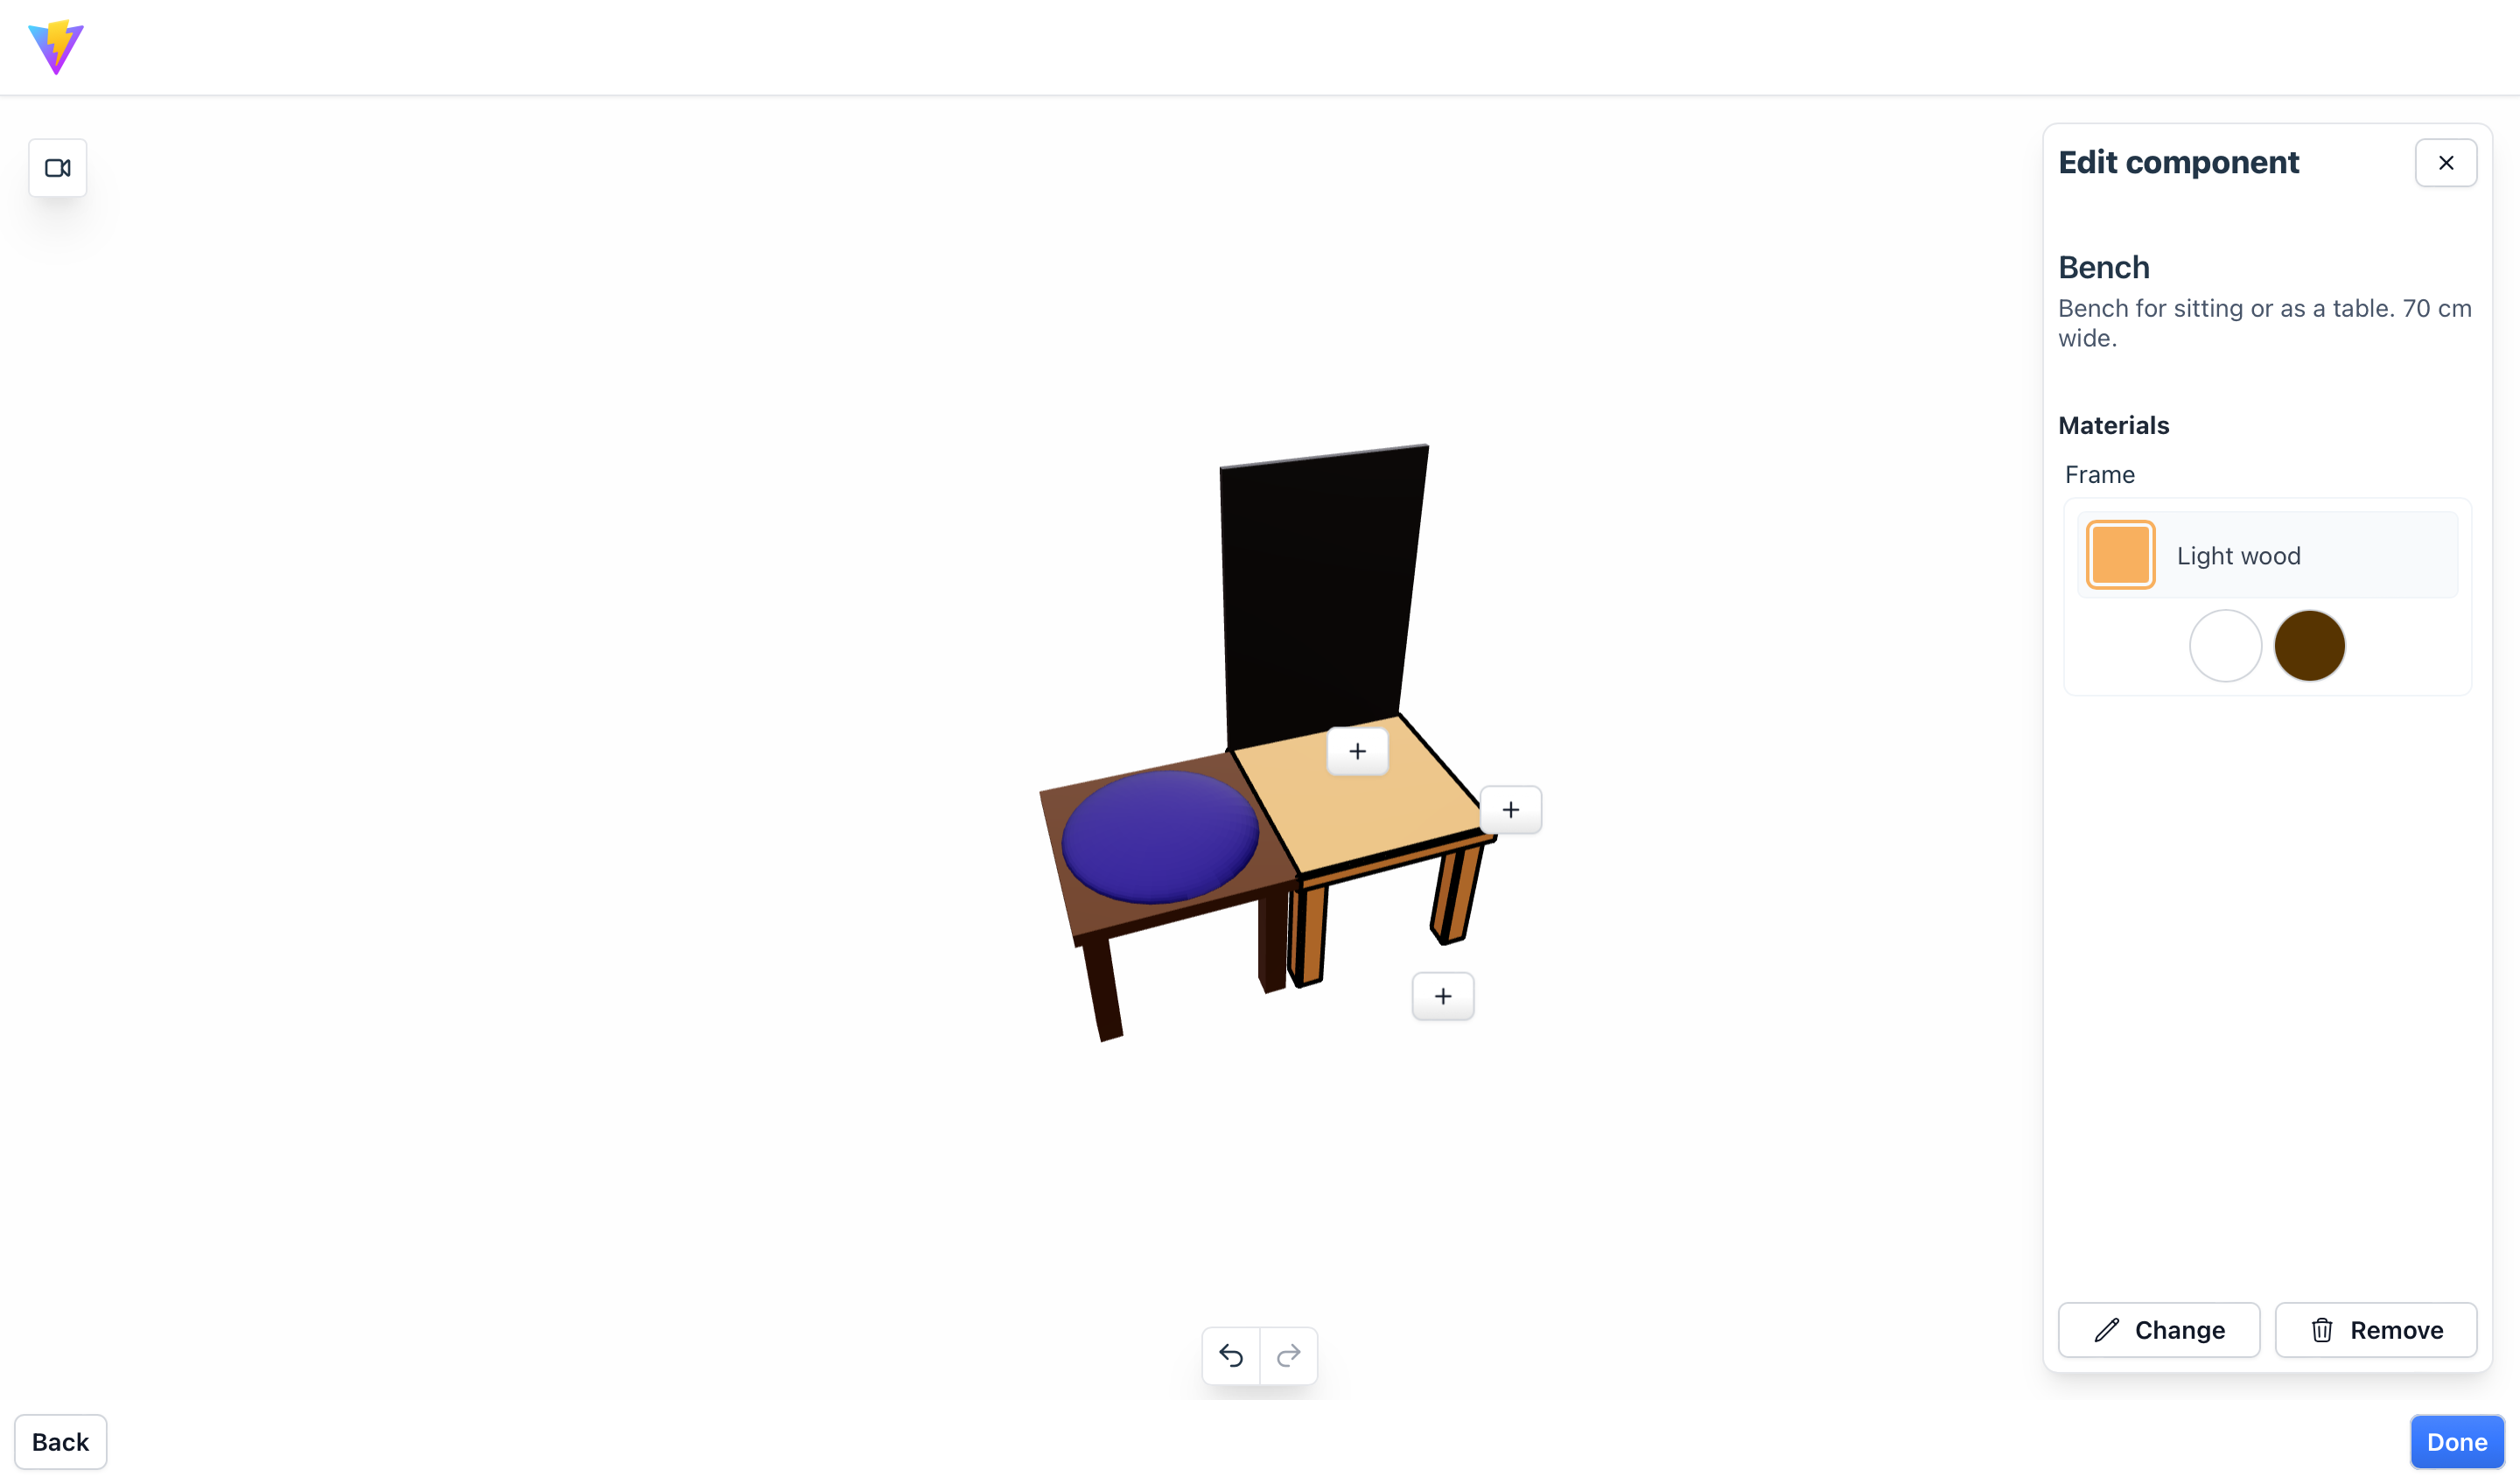
\includegraphics[width=\textwidth]{images/screenshot_configurator.png}
\caption{Screenshot of configuration screen}
\label{fig:screenshot-configuration}
\end{figure}

\subsubsection{Confirmation screen}

The implementation of the confirmation screen again closely follows the designed wireframe, as shown in \autoref{fig:screenshot-confirmation}.

The screenshot contains a list of configured components for a mocked product, each displaying the details in the form of selected color of their material.

The panel on the right side, which contains the different buttons, is floating; therefore, it stays fixed in the same position even if the page is scrolled. The panel contains back and confirm buttons, as well as a button for printing the component list visible on the left.

\begin{figure}[h]
\centering
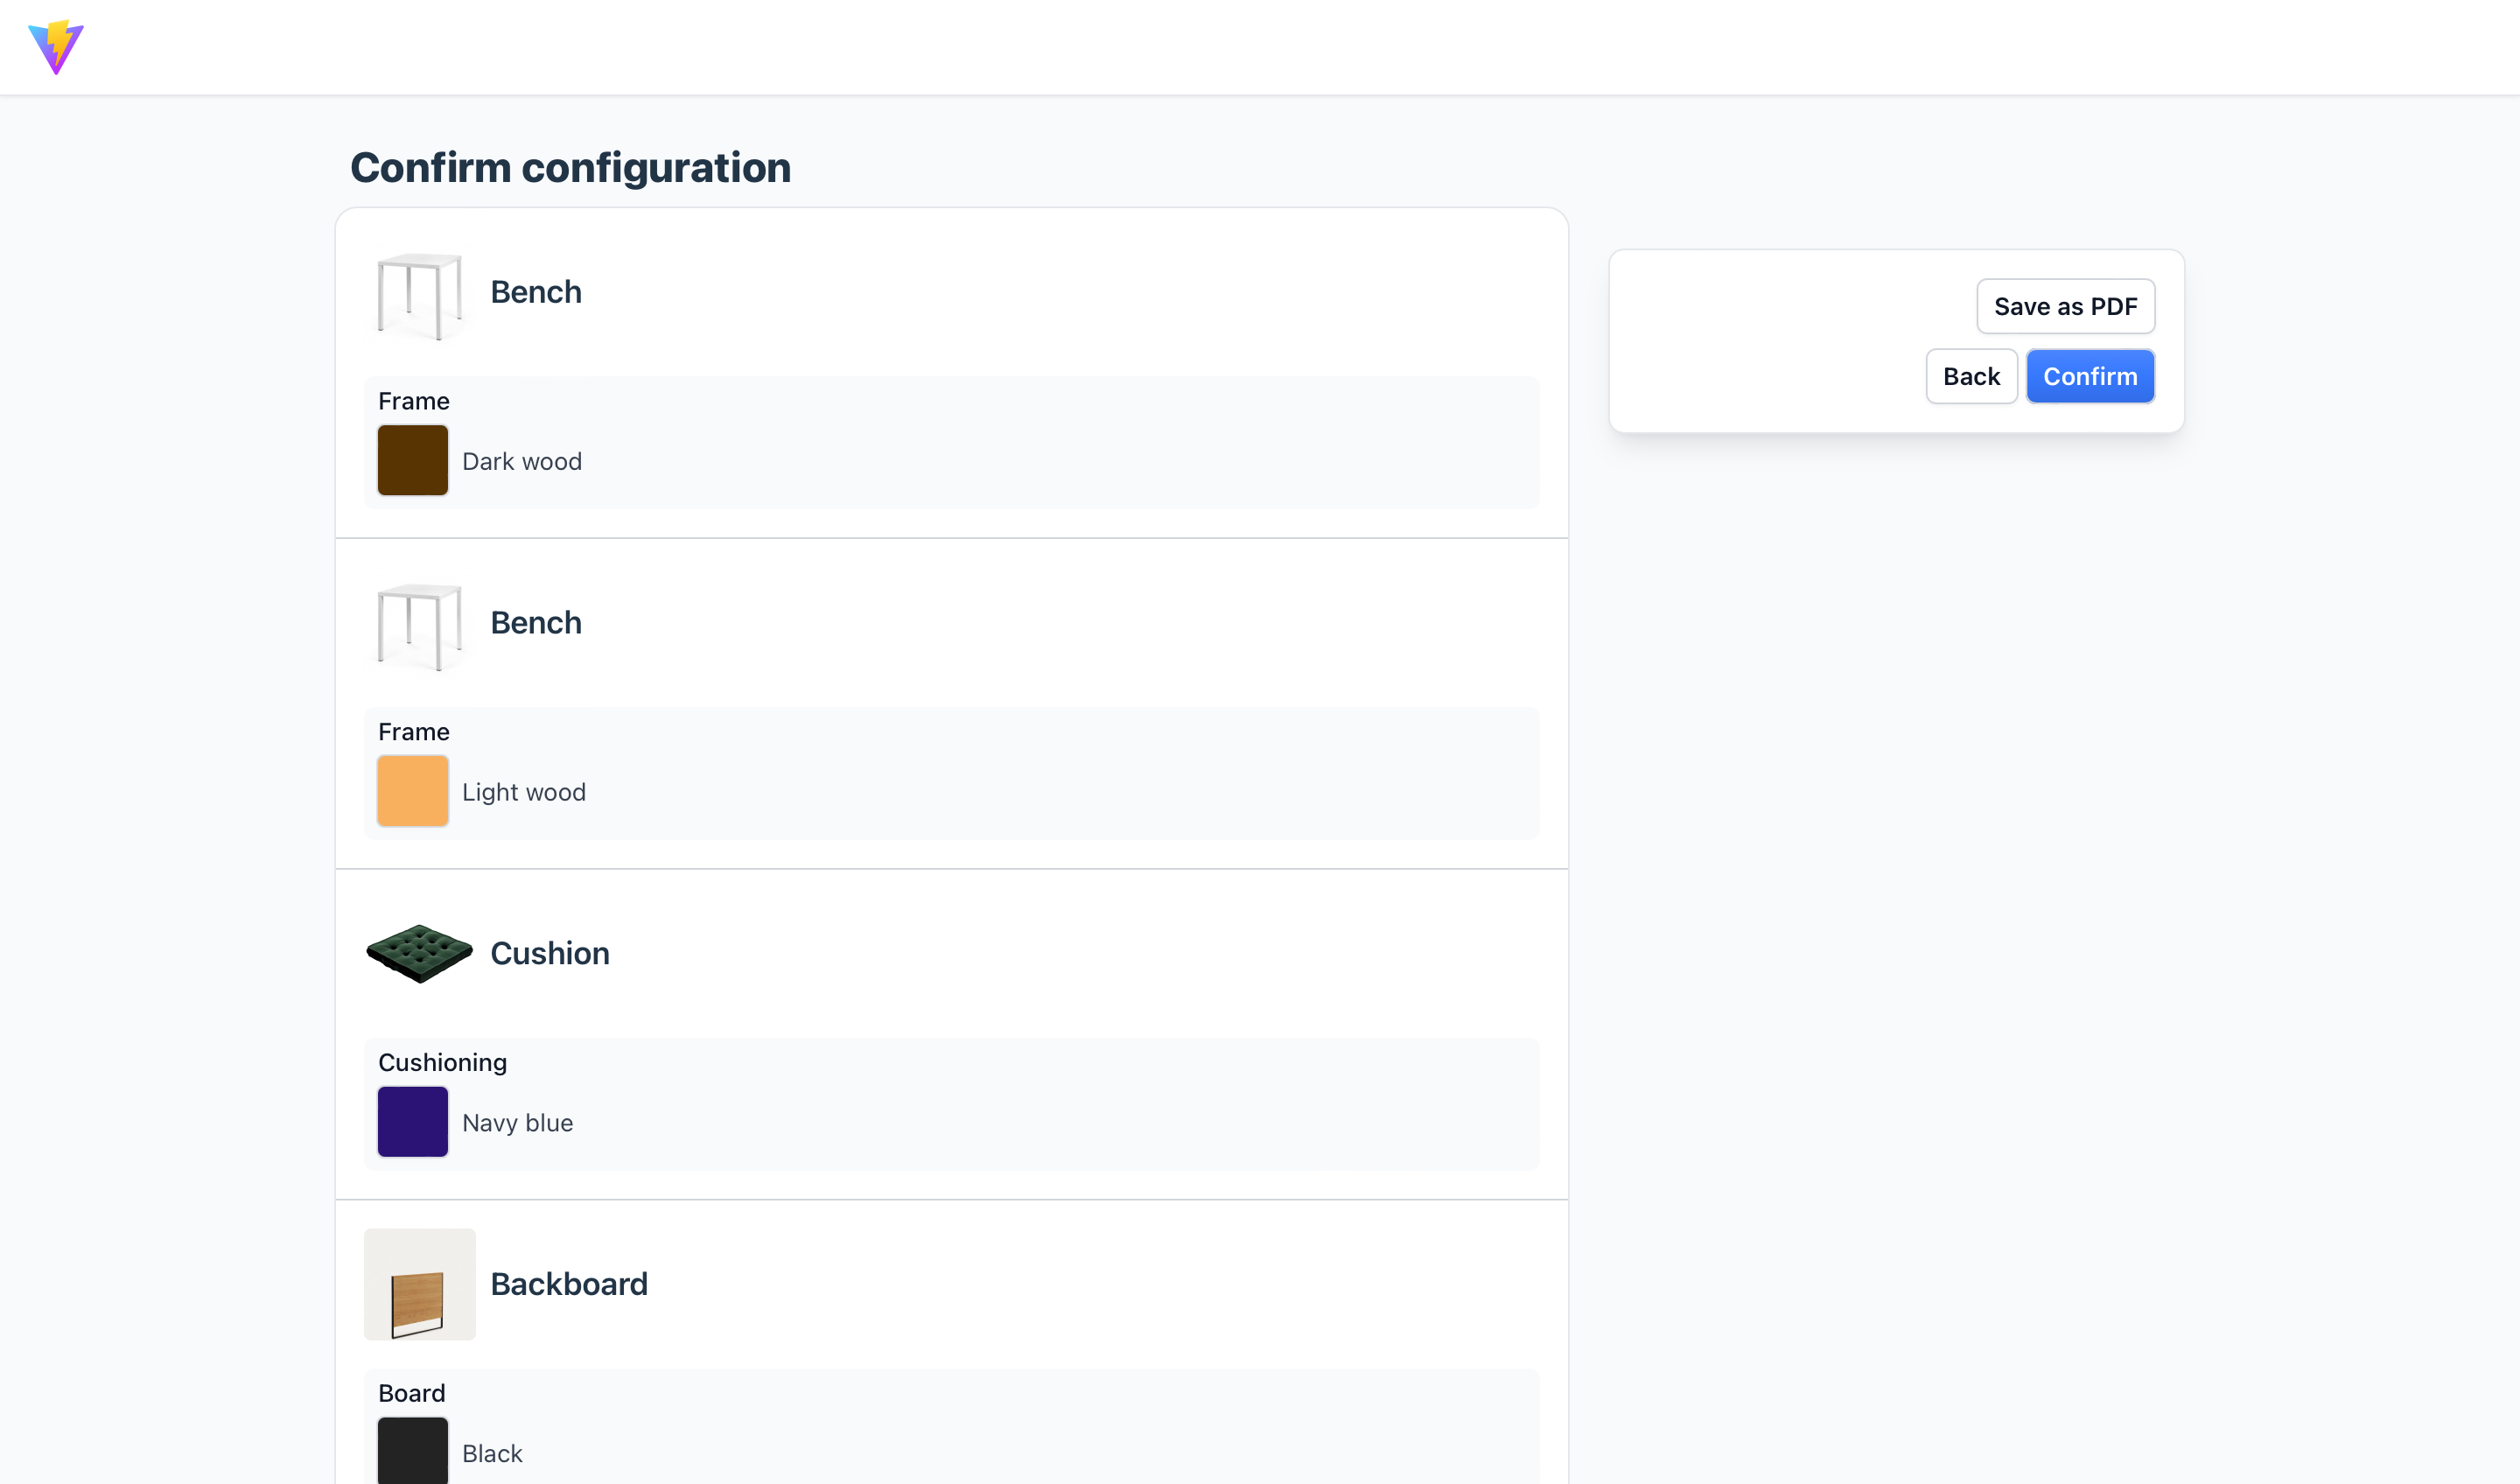
\includegraphics[width=\textwidth]{images/screenshot_confirmation.png}
\caption{Screenshot of confirmation screen}
\label{fig:screenshot-confirmation}
\end{figure}

\subsection{Administrator application}

This section presents the interfaces of the administrator application, which is described in more detail in the previous sections (see \autoref{section:catalog-management}).

\subsubsection{Catalog composer}

\begin{figure}[h]
\centering
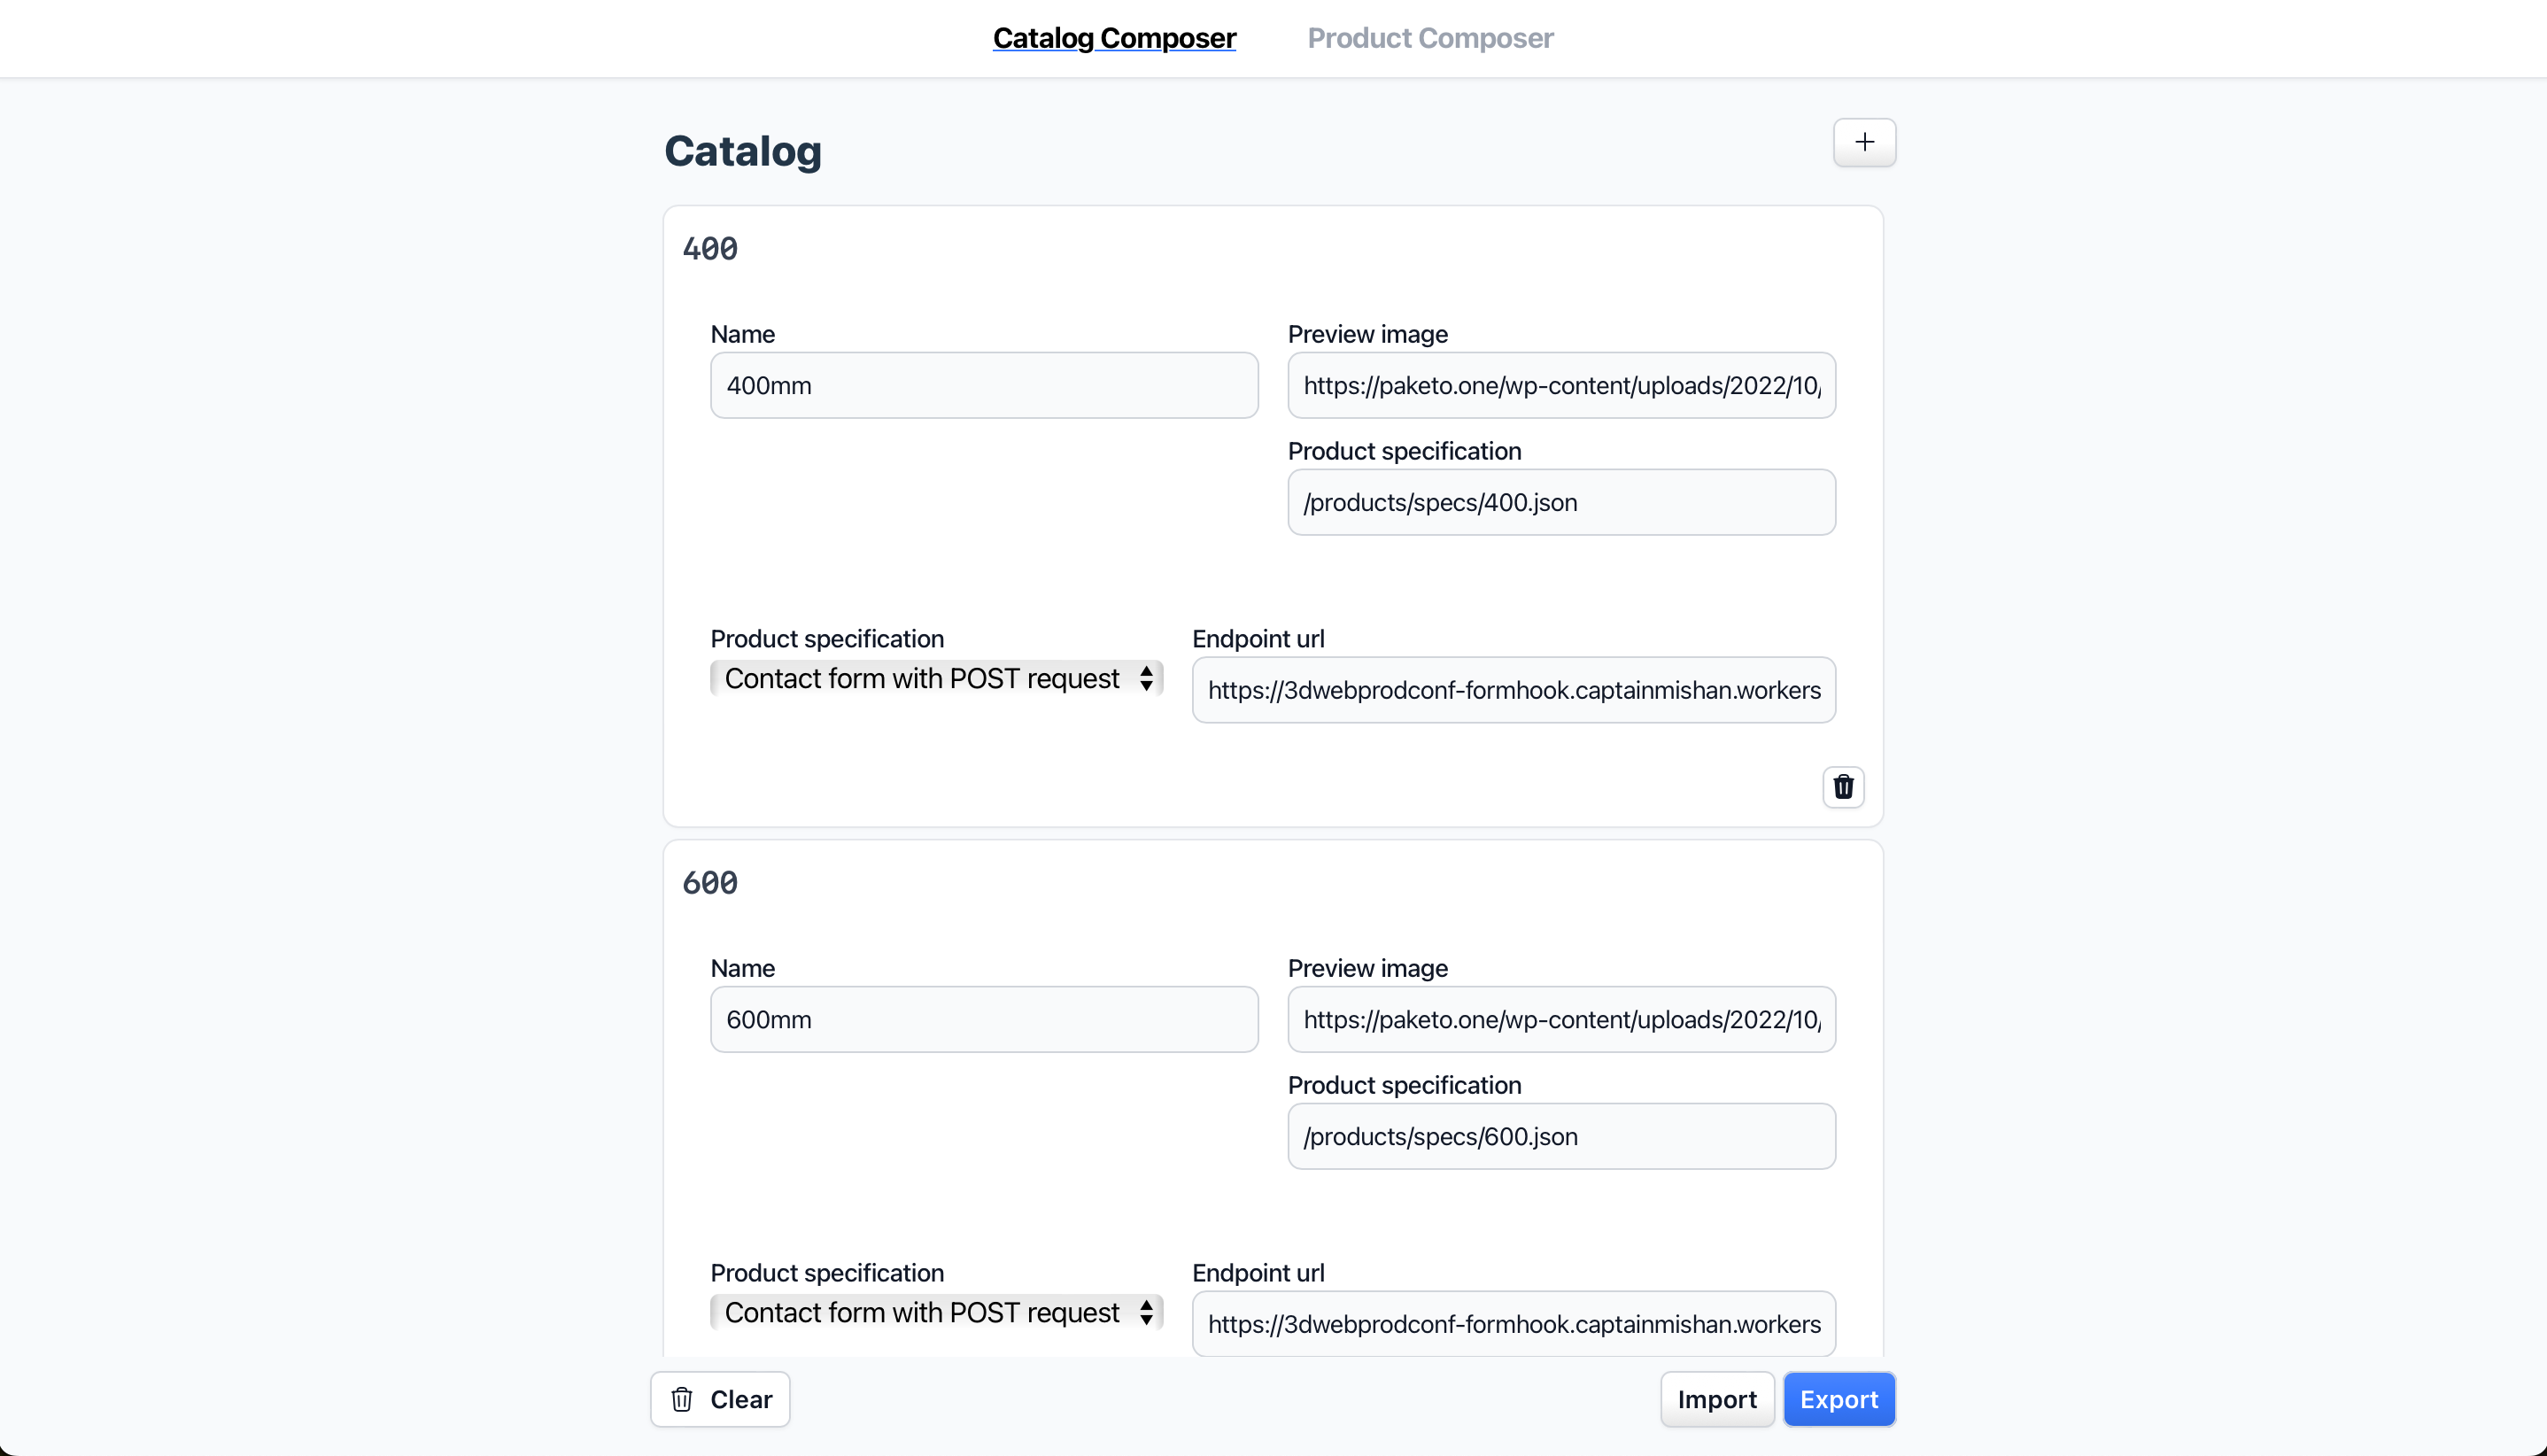
\includegraphics[width=\textwidth]{images/screenshot_catalogcomposer.png}
\caption{Screenshot of catalog composer screen}
\label{fig:screenshot-catalogcomposer}
\end{figure}

\subsubsection{Product composer}

\begin{figure}[h]
\centering
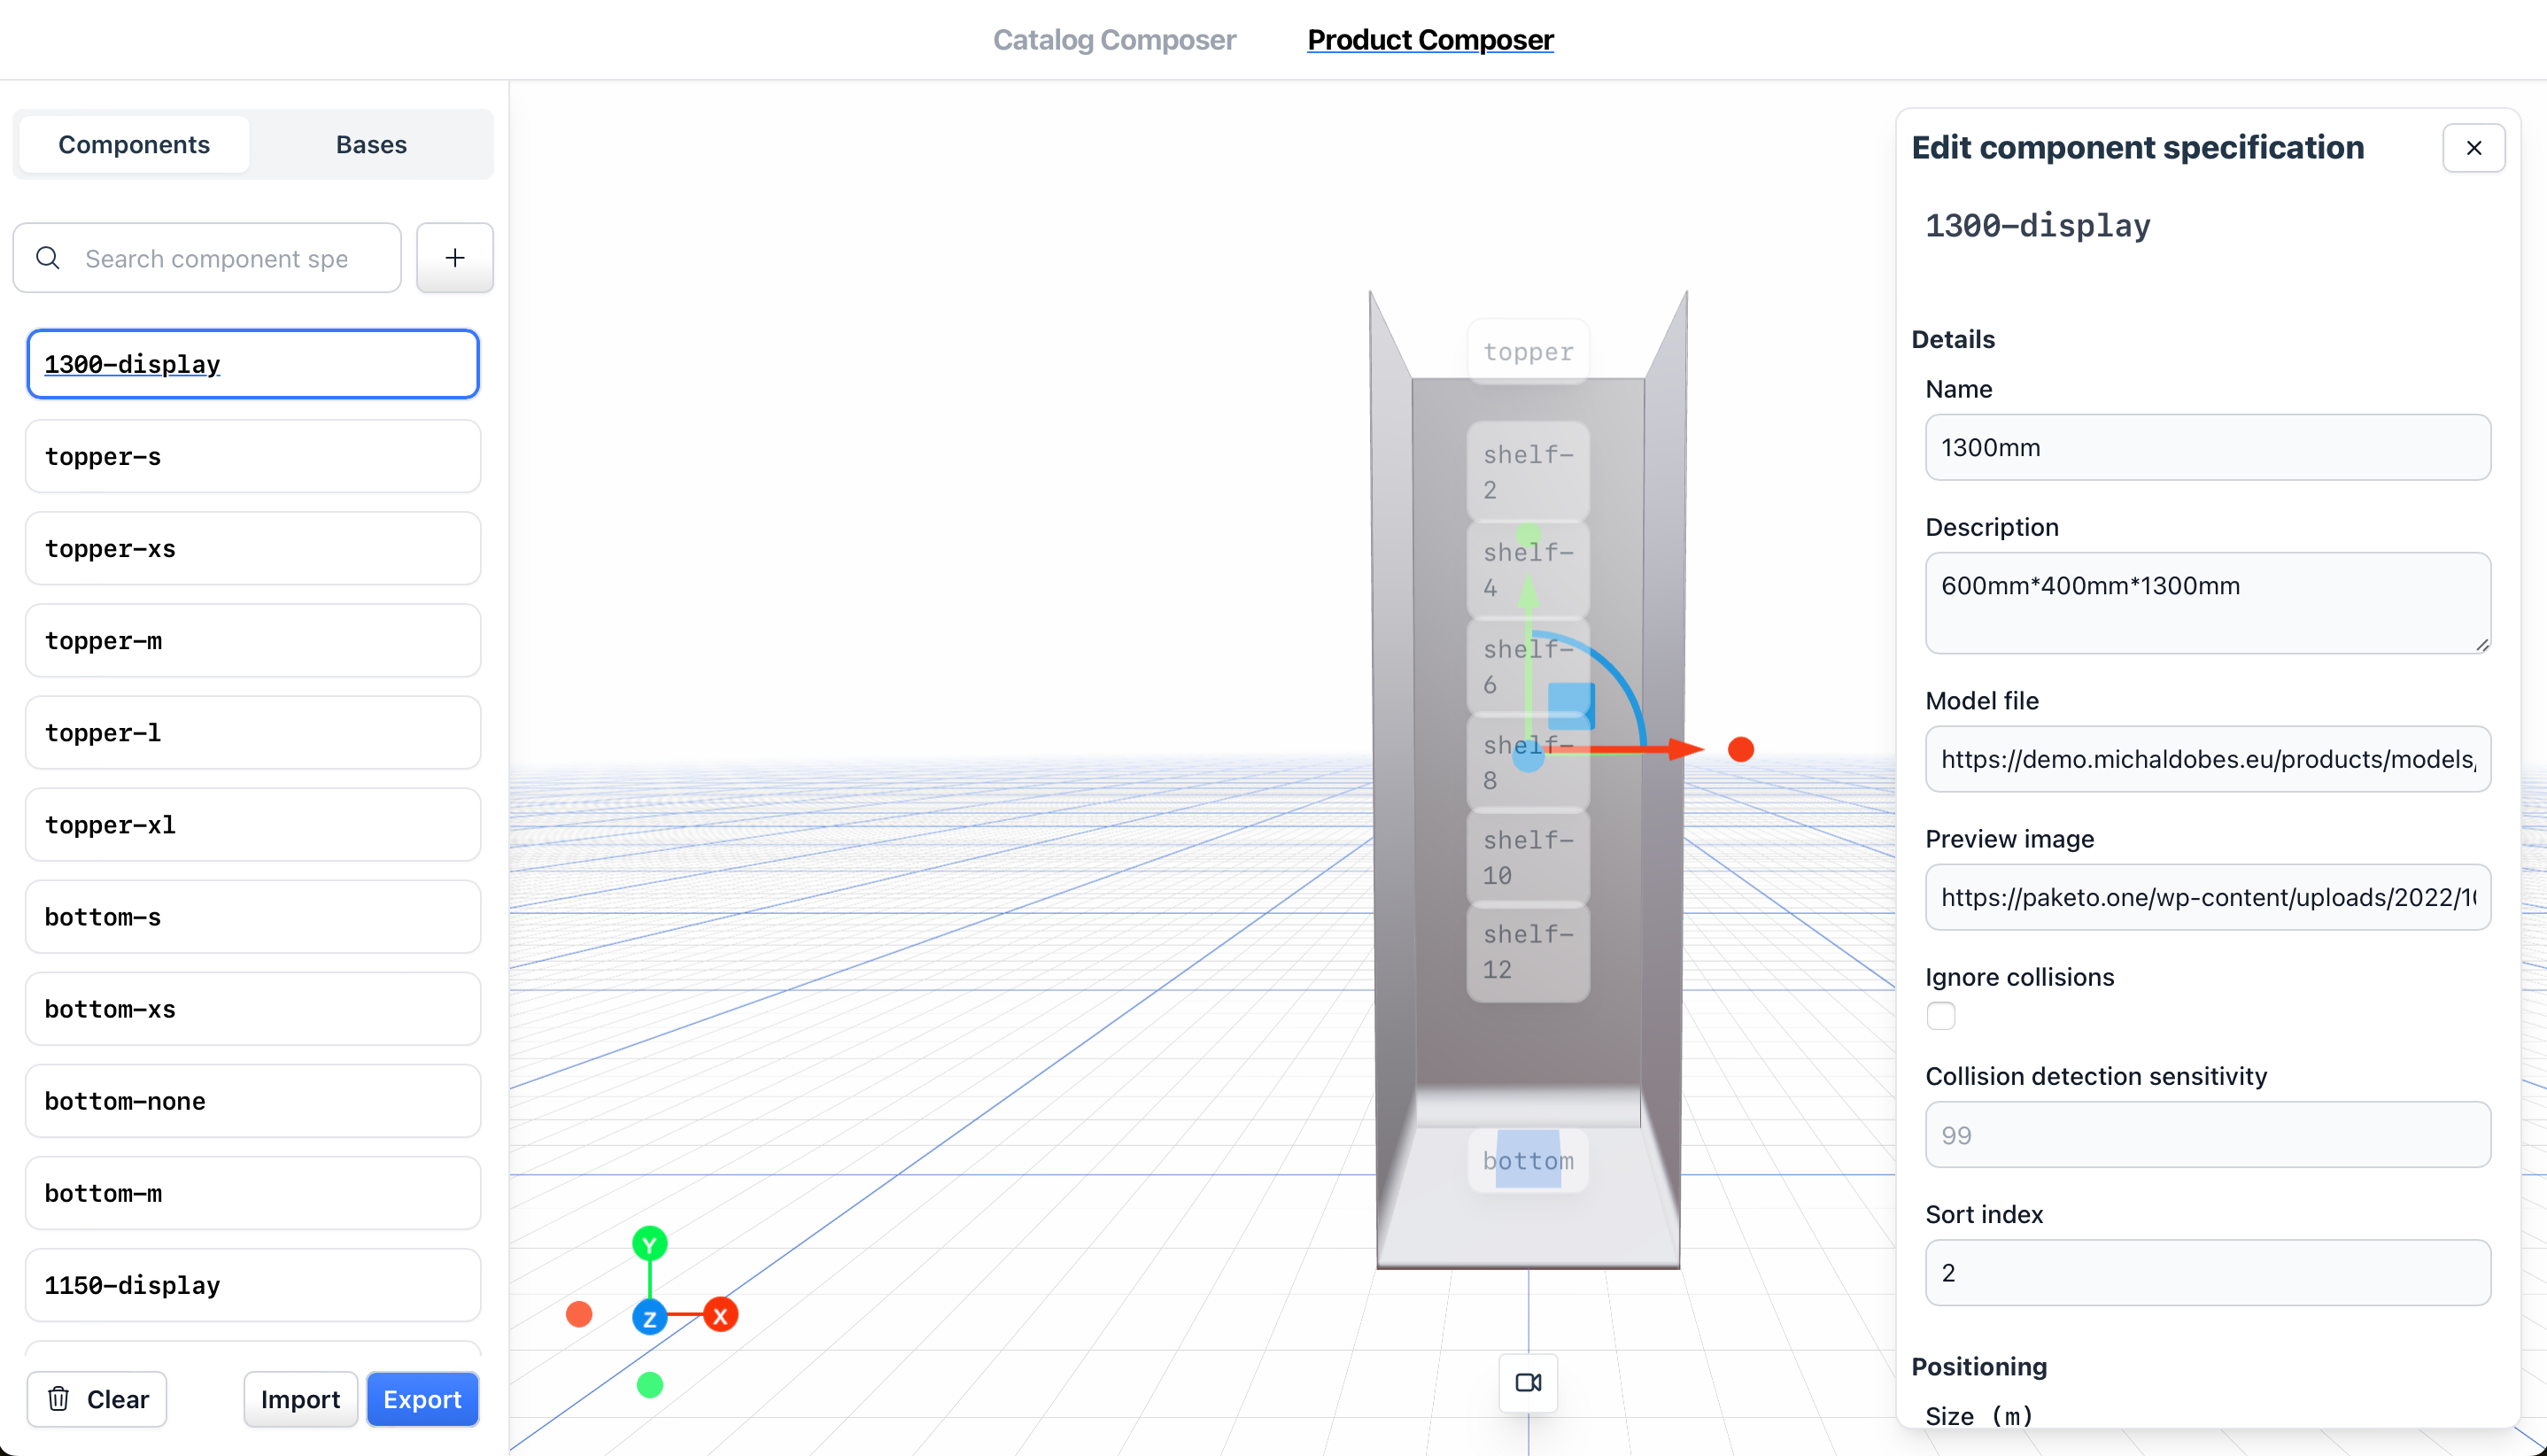
\includegraphics[width=\textwidth]{images/screenshot_productcomposer.png}
\caption{Screenshot of product composer screen}
\label{fig:screenshot-produtcomposer}
\end{figure}

\section{Summary of implementation}